%
% kreise.tex
%
% (c) 2023 Prof Dr Andreas Müller
%
\begin{figure}
\centering
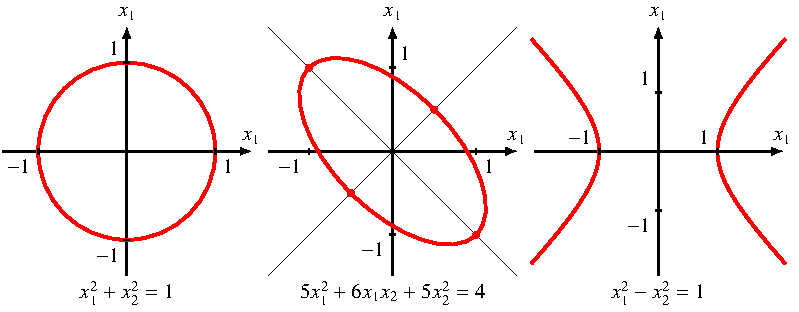
\includegraphics{chapters/010-skalarprodukt/images/kreise.pdf}
\caption{Kreise verschiedener Skalarprodukte in der Ebene.
Links der Kreis, der aus dem Standardskalarprodukt entsteht.
Rechts der zum hyperbolischen Skalarprodukt behörige ``Kreis'', er
besteht aus zwei Hyperbelästen.
Im Allgemeinen ist die Menge $\|v\|=1$ für die zu einem Skalarprodukt
gehörige Norm eine Ellipse, wie im mittleren Bild dargestellt.
\label{buch:skalarprodukt:definition:fig:kreise}}
\end{figure}
